%%%%%%%%%%%%%%%%%%%%%%%%%%%%%%%%%%%%%%%%%

%
% Important note:
% This template requires the resume.cls file to be in the same directory as the
% .tex file. The resume.cls file provides the resume style used for structuring the
% document.

%
% Creator Peilin Li
% Contact me via twitter/wechat: @pe1l1nl1
% linkedin.com/peill and/or github/ppeill
% Inspired by Peppa Pig 
%%%%%%%%%%%%%%%%%%%%%%%%%%%%%%%%%%%%%%%%

%----------------------------------------------------------------------------------------
%	PACKAGES AND OTHER DOCUMENT CONFIGURATIONS
%----------------------------------------------------------------------------------------

\documentclass{resume} % Use the custom resume.cls style

\usepackage[left=0.40in,top=0.3in,right=0.75in,bottom=0.1in]{geometry} % Document margins
\usepackage{fontawesome5}
\usepackage{academicons}
\usepackage[normalem]{ulem}
\usepackage{times}
\usepackage{etaremune}
\newcommand{\tab}[1]{\hspace{.2667\textwidth}\rlap{#1}}
\newcommand{\itab}[1]{\hspace{0em}\rlap{#1}}
\usepackage{hyperref}
\hypersetup{
        pdftoolbar=false,        	% show Acrobat’s toolbar?
        pdfmenubar=false,        	% show Acrobat’s menu?
        pdffitwindow=false,     	% window fit to page when opened
        pdfstartview={FitH},    	% fits the width of the page to the window
        pdftitle={},    	% title
        pdfauthor={},     	% author
        colorlinks=true,       	% false: boxed links; true: colored links
        linkcolor=black,          	% color of internal links (change box color with linkbordercolor)
        citecolor=black,       	% color of links to bibliography
        filecolor=black,      	% color of file links
        urlcolor=black		% color of external links
    }
\usepackage{kotex}
\usepackage{multirow}
\usepackage{graphicx}

% \begin{center}

% \end{center}

\name{
    Myeongseok Ryu
} % Your name 

\address{
    \faHome{ \href{https://kaist-mic-lab.github.io}{https://kaist-mic-lab.github.io}}
    \faOrcid{ \href{https://orcid.org/0009-0004-3279-5765}{0009-0004-3279-5765}}
    \faGithub{ \href{https://github.com/DDingR}{github.com/DDingR}} 
    } 

\address{
    \faMapMarker{ 
        \href{https://maps.app.goo.gl/R9xKhqfr56iTe5Pa6}{193, Munji-ro, Yuseong-gu, Daejeon, 34051, Korea}
    } \faPhone{
        \href{tel:+821099536538}{+82 10-9953-6538} % Your phone number
    }
    \faEnvelope{ 
        \href{mailto:dding_98@kaist.ac.kr}{dding\_98@kaist.ac.kr}
    }
    } % Your address

\begin{document}
{
    \centerline {
        \em \textbf { Myeongseok Ryu is under Ph.D. course.} (compiled on \today)
    } 
}

% ============================================
% Research Interests
% ============================================
\begin{minipage}[t]{0.5\textwidth}
    \begin{rSection}{Research Interests}
    \vspace{.5em}
    \small{
        {\bf Control Theory} 
        \\
        Adaptive Control, Optimal Control

        \vspace{.5em}
        {\bf Neural Network-based Control} 
        \\
        Neuro-Adaptive Control, Reinforcement Learning

        \vspace{.5em}
        {\bf Contraction Theory} 
        
        \vspace{.5em}
        {\bf Online Optimization}
    }
    \end{rSection}
\end{minipage}
\hfill
\begin{minipage}[t]{0.35\textwidth}
    \begin{rSection}{Profile \& Logos}
        \vspace{.5em}
        \begin{center}
            \begin{tabular}{cc}
                \multirow{3}{*}{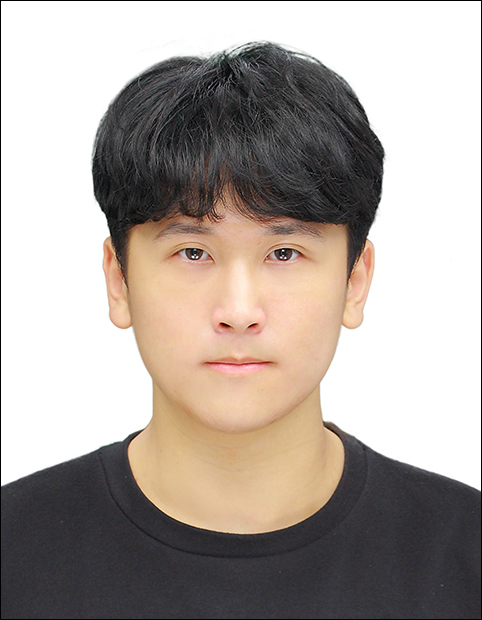
\includegraphics[width=0.4\textwidth]{ms.jpg}}\vspace{1em} &
                \\
                [-.5em]
                & 
                
\includegraphics[width=0.4\textwidth]{logo_KAIST_simple.png}
                \\
                [1em]
                & 
                
\includegraphics[width=0.4\textwidth]{logo_MIC.png} \\
            \end{tabular}
        \end{center}
    \end{rSection}
\end{minipage}

% ============================================
% Education
% ============================================
\begin{rSection}{Education}

\small{
    {\bf Korea Advanced Institute of Science and Technology (KAIST), Korea}
        \hfill 
        {\em September 2025 – Present} 
        \\
        CCS Graduate School of Mobility
        \\
        {\textit {Ph.D. of Science in Mobility Engineering}} 
        \vspace{-.5em}
        \begin{itemize}
            \item Supervisor: Prof. Kyunghwan Choi, KAIST
        \end{itemize}

    \sout{\bf{Gwangju Institute of Science and Technology (GIST), Korea}}, (\textit{Withdrew for further studies})
        \hfill 
        {\em March 2025 – May 2025} 
        \\
        \sout{School of Mechanical Engineering}
        \\
        \sout{\textit {Ph.D. of Science in Mechanical Engineering}} 

    {\bf Gwangju Institute of Science and Technology (GIST), Korea} 
        \hfill 
        {\em March 2023 – February 2025} 
        \\
        School of Mechanical Engineering
        \\
        {\textit {Master of Science in Mechanical Engineering}} 
        \vspace{-.5em}
        \begin{itemize}
            \item Thesis: Constrained Optimization-Based Neuro-Adaptive Control (CoNAC) for Euler-Lagrange Systems
            \vspace{-.75em}
            \item Supervisor: Prof. Kyunghwan Choi, GIST
        \end{itemize}

    {\bf Incheon National University (INU), Korea} 
        \hfill 
        {\em March 2017 – February 2023} 
        \\
        Department of Mechanical Engineering
        \\
        {\textit {Bachelor of Engineering}} 
}


\end{rSection}

% ============================================
% Professional Experience
% ============================================
\begin{rSection}{Professional Experience}

\small{

    {\bf Korea Advanced Institute of Science and Technology (KAIST), Korea}
    \hfill 
    {\em May 2023 – August 2025} 
    \\
    {\textit {Part time Contract Research Scientist}}
    \\
    - Research on Neural Network-based Control for Mobility Systems

}

\end{rSection}

% ============================================
% Skills
% ============================================
\begin{rSection}{Skills}

\small{

\begin{tabular}{ @{} >{\bfseries}l @{\hspace{6ex}} l }
    Languages: \ & Korean, English \\

    Programming: \ & Matlab/Simulink, Python, C/C++ \\

    Implementation: 
        & {\textbf{Simulation }}CarMaker, ROS
        \\
        & {\textbf{Others }}Git, LaTeX, Jekyll
\end{tabular}

}

\end{rSection}

% ============================================
% Publications
% ============================================
\begin{rSection}{Publications}


\textbf{International Journal Papers}

\small{\begin{etaremune}

    \item {
        Constrained Optimization-Based Neuro-Adaptive Control (CONAC) for Euler-Lagrange Systems Under Weight and Input Constraints
        \\
        \textbf{Myeongseok Ryu}, Donghwa Hong, Kyunghwan Choi*
        \\
        \textit{
            IEEE Transactions on Cybernetics, 2025
        }
    }

\end{etaremune}}
    
\textbf{International Conference Papers}

\small{\begin{etaremune}

    \item {
        \href{https://doi.org/10.36227/techrxiv.172893538.89561848/v1}{Physics-Informed Online Learning of Flux Linkage Model for Synchronous Machine}
        \\
        Seunghun Jang, \textbf{Myeongseok Ryu}, Kyunghwan Choi*
        \\
        \textit{
            IEEE IECON, (accepted, in press), 2025
        }
    }

    \item {
        \href{https://doi.org/10.36227/techrxiv.174585949.94234666/v1}{Constrained Optimization-Based Neuro-Adaptive Control (CONAC) for Synchronous Machine Drives Under Voltage Constraints}
        \\
        \textbf{Myeongseok Ryu}, Niklas Monzen, Pascal Seitter, Kyunghwan Choi, Christoph M. Hackl*
        \\
        \textit{
            IEEE IECON, (accepted, in press), 2025
        }
    }

    \item {
        \href{https://doi.org/10.36227/techrxiv.173014412.26480551/v1}{Imposing a Weight Norm Constraint for Neuro-Adaptive Control}
        \\
        \textbf{Myeongseok Ryu}, Jiyun Kim, Kyunghwan Choi*
        \\
        \textit{
            European Control Conference (ECC), (accepted, in press), pp. 380-385, 2025
        }
    }

    \item {
        \href{https://doi.org/10.1109/IWIS58789.2023.10284677}{A Comparative Study of Reinforcement Learning and Analytical Methods for Optimal Control}
        \\
        \textbf{Myeongseok Ryu}, Junseo Ha, Minji Kim, Kyunghwan Choi*
        \\
        \textit{
            International Workshop on Intelligent Systems (IWIS), pp. 1-5, 2023
        }
    }

\end{etaremune}}
    
\textbf{Domestic Conference Papers}

\small{\begin{etaremune}

    \item {
        \href{https://www.dbpia.co.kr/journal/articleDetail?nodeId=NODE11909146}{Approximation-based Steering Controller with Deep Neural Network}
        \\
        \textbf{Myeongseok Ryu}, Kyunghwan Choi*
        \\
        \textit{
            제어로봇시스템학회 (ICROS), pp. 884-885, 2024
        }
    }

    \item {
        \href{https://www.dbpia.co.kr/journal/articleDetail?nodeId=NODE11665897}{Integrated Motion Control of Four in-Wheel Motor Actuated Vehicles Considering Path Tracking, Ride Comfort, and Energy Efficiency}
        \\
        \textbf{Myeongseok Ryu}, Kyunghwan Choi*
        \\
        \textit{
            한국자동차공학회 추계학술대회 (KSAE), pp. 490, 2023
        }
    }

    \item {
        \href{https://www.dbpia.co.kr/journal/articleDetail?nodeId=NODE11480596}{Data-driven Modeling of Model Residuals for Linear Model Predictive Control of Nonlinear Systems}
        \\
        \textbf{Myeongseok Ryu}, Kyunghwan Choi*
        \\
        \textit{
            제어로봇시스템학회 (ICROS), pp. 837-838, 2023
        }
    }

\end{etaremune}}
    
\textbf{Preprint Papers}

\small{\begin{etaremune}

    \item {
        \href{https://doi.org/10.48550/arXiv.2403.03499}{CNN-based End-to-End Adaptive Controller with Stability Guarantees}
        \\
        \textbf{Myeongseok Ryu}, Kyunghwan Choi*
        \\
        \textit{
            Arxiv, 2024
        }
    }

\end{etaremune}}
    

\end{rSection}

% ============================================
% Grants and Awards
% ============================================
\begin{rSection}{Grants and Awards}

\small{

    {\bf IEEE International Workshop on Intelligent Systems (IWIS)} 
        \hfill 
        {\em July 2025} 
        \\
        {\textit {Best Presentation Paper Award}} 

    {\bf European Control Association (EUCA) } 
        \hfill 
        {\em June 2025} 
        \\
        {\textit {Student Support}}
        \hfill 
        {400 EUR}

    {\bf Graduate International Research Experience Fellowship (GIST-IREF)} 
        \hfill 
        {\em October 2024} 
        \\
        {\textit {Research Support}}
        \hfill 
        {16 million KRW (approx. 12,000 USD)}
        
    {\bf Institute of Control, Robotics and Systems (ICROS)} 
        \hfill 
        {\em June 2023} 
        \\
        {\textit {Best Paper Award}} 

    {\bf INU MATLAB Cody Challenge} 
        \hfill 
        {\em June 2021} 
        \\
        {\textit {Top Prize}} 

}

\end{rSection}

\end{document}